\documentclass[spanish]{udpreport}
\usepackage[utf8]{inputenc}
\usepackage[spanish]{babel}

% Podemos establecer el logo de alguna entidad o dejar el de la UDP (defecto)
%\setlogo{EITFI}

\title{Informe Laboratorio III \\ Redes de Datos}
\author{Arturo Mantinetti \\ Manuel Tobar \\ Diego Vilches \\ Nicolas Henriquez}
\email{arturo.mantinetti@mail.udp.cl \\ manuel.tobar@mail.udp.cl
	\\ diego.vilches@mail.udp.cl \\ nicolas.henriquez@mail.udp.cl}
	
\profesor{Profesor \\ Jaime Álvarez}
\ayudante{Ayudante \\ Maximiliano Vega}


\date{14 de Abril de 2016}

% Además podemos establecer la facultad y escuela
% los valores por defecto son los siguientes:
%\udpschool{Escuela de Informática y Telecomunicaciones}
%\udpfaculty{Facultad de Ingeniería}
%\udpuniversity{Universidad Diego Portales}

\begin{document}
\maketitle

\tableofcontents

\chapter{Introducción}

Este laboratorio consistió en crear paquetes de datos con diferentes parámetros para luego enviarlos por la red, con el fin lo lograr comprender como se conforman y comportan estos según sus características. Esto es posible gracias a un programa llamado 'Scapy' que nos da esas funcionalidades. 

Los paquetes, en este experimento, varían principalmente en la dirección MAC, lo que hace que sean recibidos por distintos equipos. Para esto se ocupa 'Wireshark', programa con el que se puede capturar los paquetes enviados por la red.  Una vez creados y enviados los paquetes a través del Switch, se repite el procedimiento, sólo que esta vez los equipos están conectados a un Hub. 



\chapter{Contenido}

\section{Creación de Paquetes}
Para crear un paquete con Scapy, este se tiene que ejecutar vía la consola el siguiente comando:

\begin{center}
	\emph{sudo scapy}
\end{center}

Este comando iniciará el programa como super-user donde se podrá usar sus funciones para la creación de los paquetes y enviarlos por la red. Estos se crean en base a las capas del modelo OSI, sin necesidad de seguir un orden especifico al crear las capas, las cuales el programa permite su uso desde la Capa 2 hasta la que se necesite para el paquete.

\begin{center}
	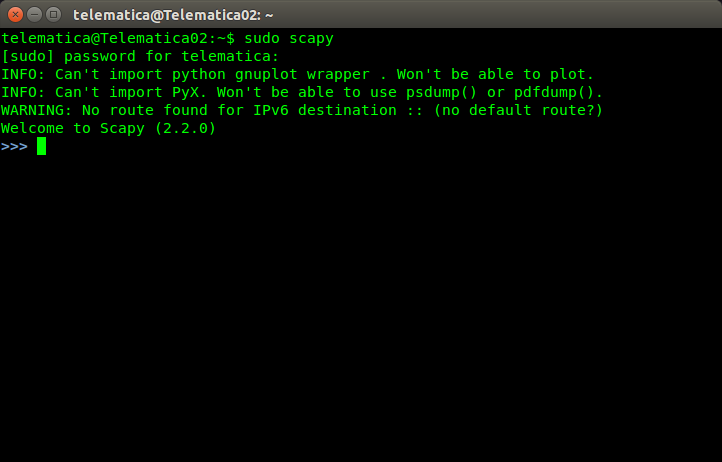
\includegraphics[scale=.37]{imagenes/Scapy_Init.png}
\end{center}

Iniciando con la Capa 2 esta el comando Ether(), este comando permite modificar los parámetros del enlace de datos, en especial las MACs de destino y origen, en este laboratorio se utiliza en demasía esta capa.


El siguiente comando, el cual se encarga de la Capa 3, es IP() el cual se encarga de los parámetros de enrutamiento incluyendo protocolos y direcciones lógicas del sistema, las direcciones de IP de origen y destino.


A continuación se define ICMP(), o Internet Control Message Protocol, el cual es un protocolo como UDP o TCP, el cual se encarga de administrar la informacion relacionada con errores de los equipos en Red, este maneja mensajes de errores y control para los sistemas de la red, informando con ellos a la fuente original para que evite o corrija el problema detectado.

El ultimo comando a usar, el cual se encarga de la información a enviar, es Raw() este se tiene un String como parámetro para el envío de información a ser usada por el equipo de destino.
\\

Una vez creadas las capas a usar, estas son apiladas en orden ascendente separadas con un '/' para que estas formen un solo paquete que luego puede ser enviado, para el envío de este se utiliza el comando sendp(), este lo envía a través de la red hacia su destino dependiendo de como este configurado.


\section{Hardware utilizado}

Para este laboratorio se utilizó una red montada con un Switch, para esto fue utilizado un Catalyst 2690 fabricado por Cisco System, y una red montada con un Hub, siendo este un AdvanceStack Switching Hub-12R fabricado por Hawlett Packard.

\begin{center}
	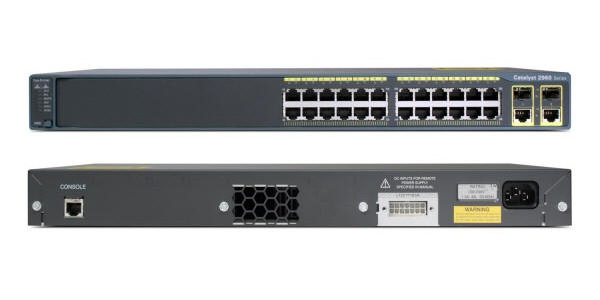
\includegraphics[scale=.5]{imagenes/Switch/switch.png}
	\includegraphics[scale=.08]{imagenes/Hub/Hub.png}
	\linebreak
\end{center}

Los equipos conectados al Switch para realizar las pruebas fueron los equipos del laboratorio de Informática, mientras que los equipos que fueron utilizados para realizar las pruebas con el Hub fueron notebooks.

\newpage


\section{Envío de un paquete de datos a FF:FF:FF:FF:FF:FF}

Se crea el paquete con la dirección MAC 'FF:FF:FF:FF:FF:FF', ante se fija el valor en el campo de destino, 'dst', con los valores dado por el ejercicio. El resto de los campos son innecesarios para la actividad por lo cual son dejados por defecto.

\begin{center}
	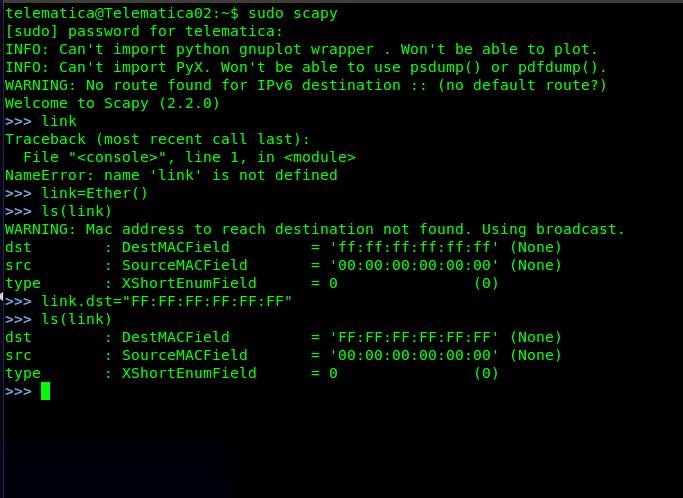
\includegraphics[scale=.37]{imagenes/Switch/Test_1a_b.png}
\end{center}

Al no necesitar ningún parámetro extra en las capas superiores solo son definidas, aunque estas no son necesarias para el funcionamiento del paquete . Solo se modifica el parámetro de la función Raw() para poder identificar el paquete enviado, una vez hecha la modificación a ese parámetro apilamos el paquete y procedemos el envío de este.

\begin{center}
	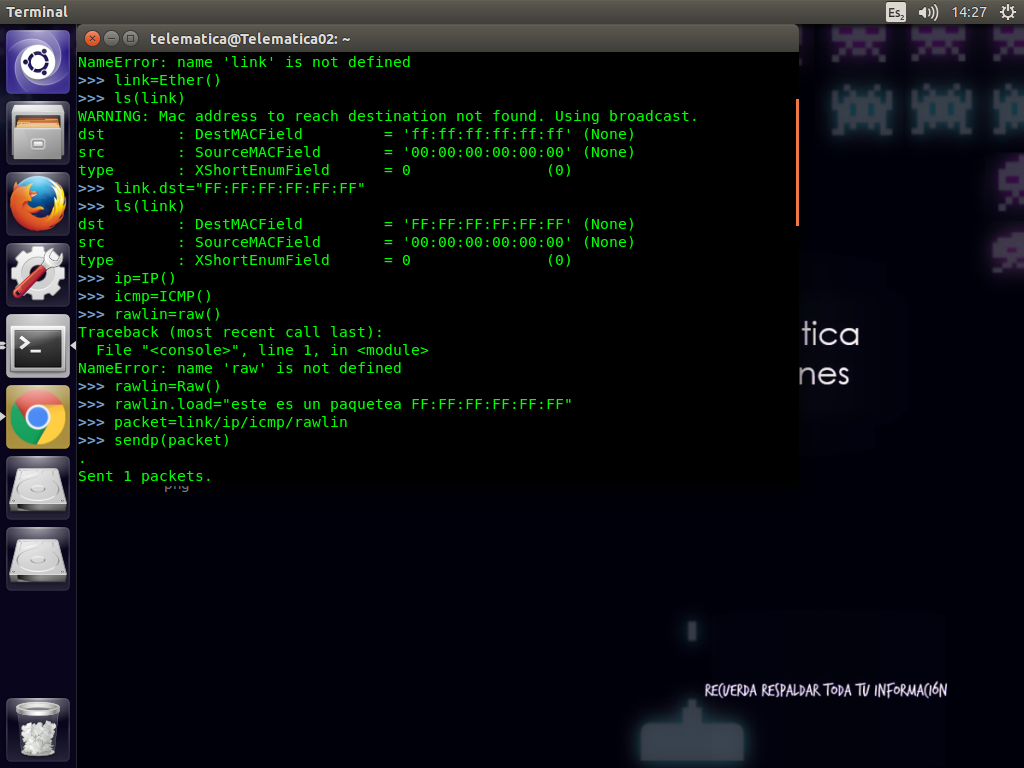
\includegraphics[scale=.37]{imagenes/Switch/Test_1b.png}
\end{center}

\pagebreak

\subsection{Switch}

Al ser la dirección MAC 'FF:FF:FF:FF:FF:FF' el Switch no reenvía el paquete a ningún equipo que se encuentre dentro de la red. Adicionalmente a esto si se usaWireshark en modo Promiscuo se puede capturar el paquete que se ha enviado.

\begin{center}
	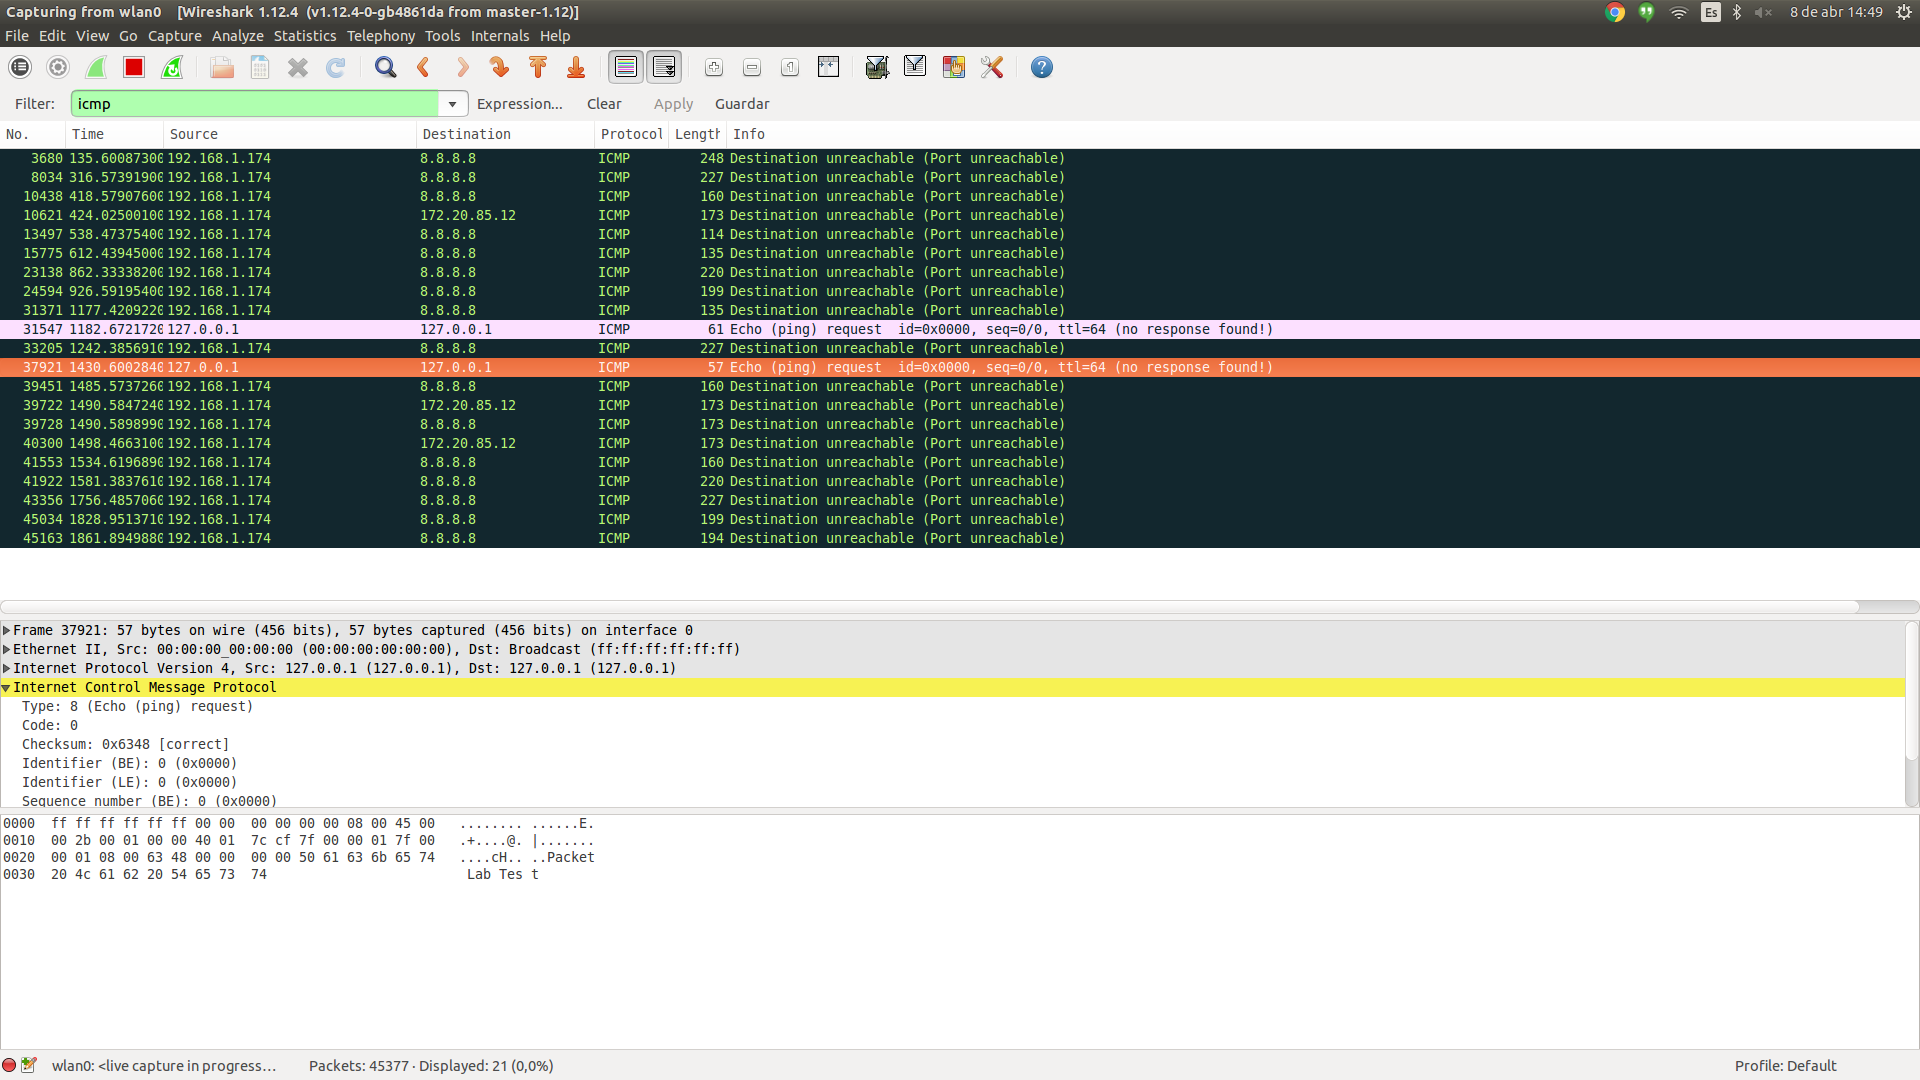
\includegraphics[scale=.21]{imagenes/Switch/FF.png}
	\\ Wireshark corriendo en Modo Promiscuo
\end{center}



\subsection{Hub}

El Hub reenvía el paquete a todos los equipos conectados a este. Siendo posible capturarlo de cualquier equipo dentro de la red sin la necesidad de correr Wireshark en modo Promiscuo, debido a que les llega a todos los equipos dentro de esta.

\begin{center}
	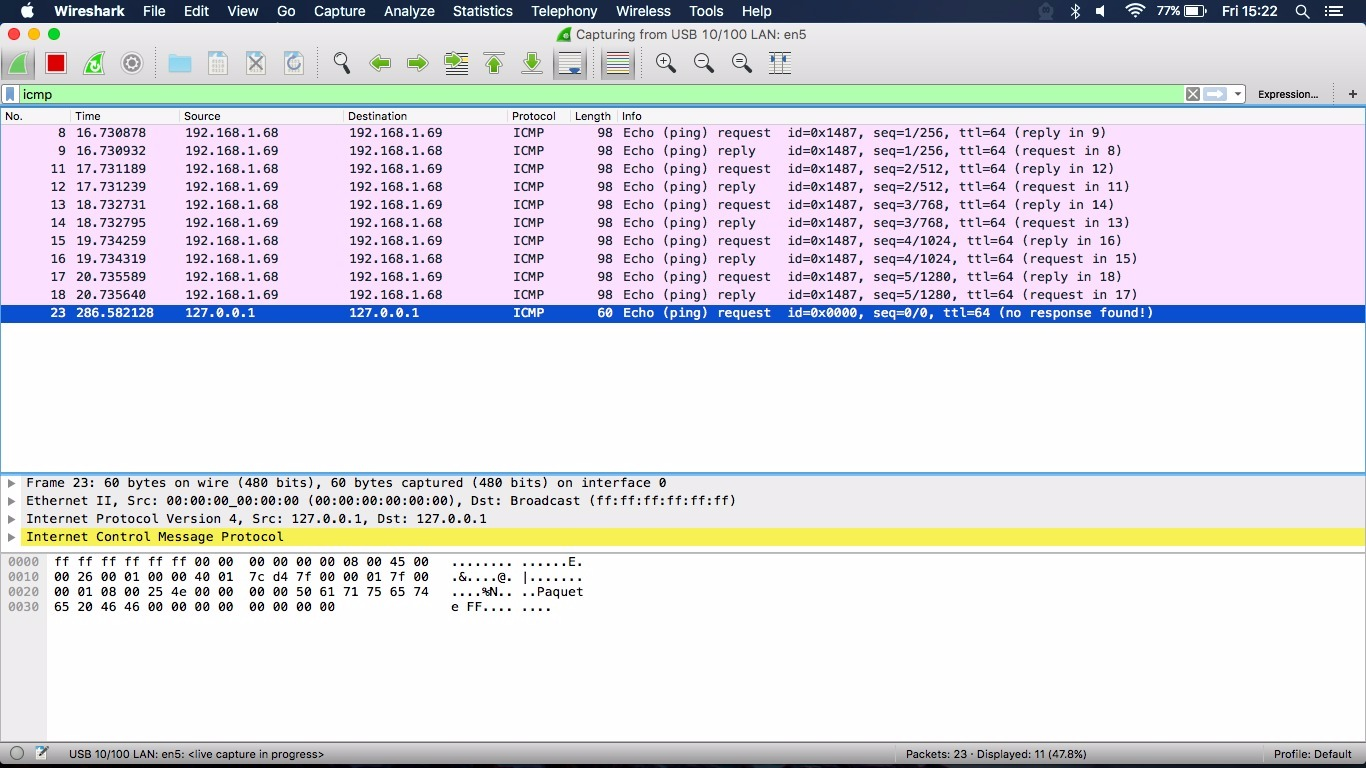
\includegraphics[scale=.3]{imagenes/Hub/FF.jpg}
\end{center}


\section{Envío de un paquete de datos con MAC especifica}

Para este segundo experimento, esta vez se usa una dirección MAC que pertenece a un equipo dentro de la red LAN, al igual que en el experimento anterior no es necesario usar parámetros adicionales de las capas superiores a excepción de la ultima capa que fue usada para identificar fácilmente nuestro paquete.

\subsection{Switch}

Para este experimento, esta vez se utilizó la siguiente dirección MAC '18:A9:05:1F:E2:5B'.
\begin{center}
	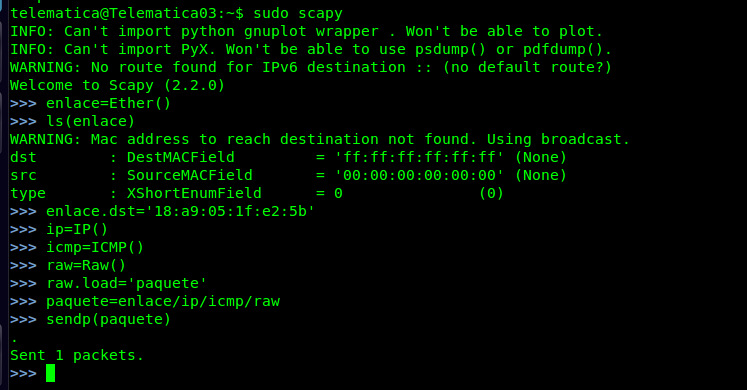
\includegraphics[scale=.37]{imagenes/Switch/Test_2.png}
\end{center}

Luego se busca en paquete en Wireshark para ver si se envió correctamente y llego a destino.

\begin{center}
	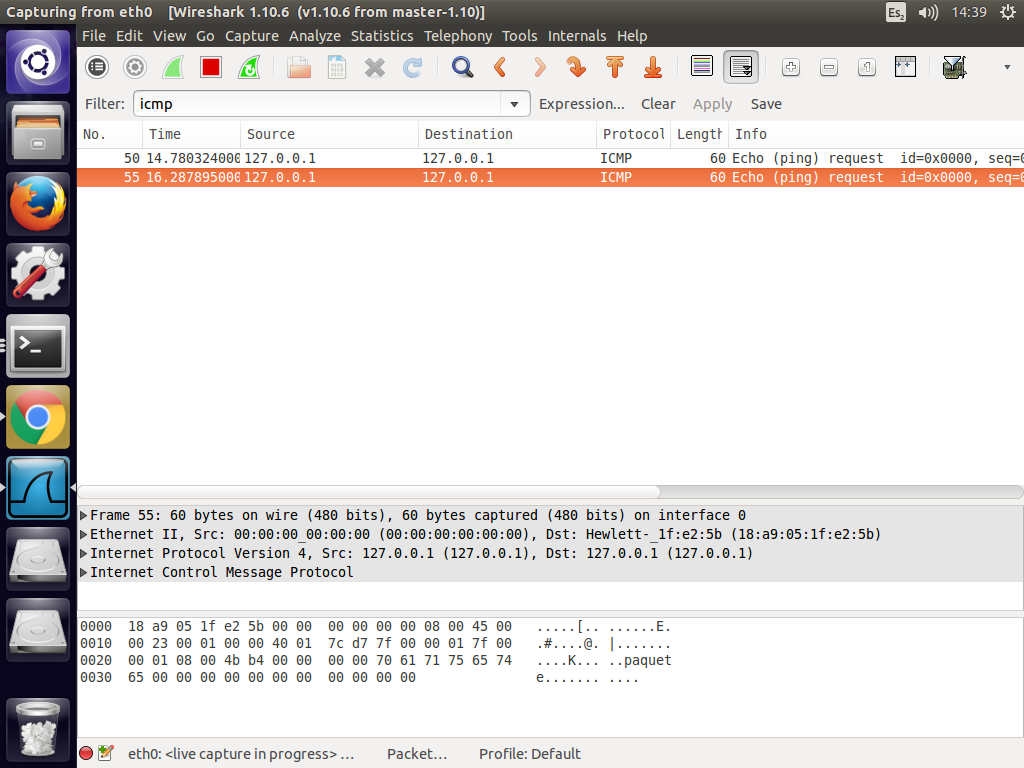
\includegraphics[scale=.37]{imagenes/Switch/Test_2_Wireshark.png}
\end{center}

\pagebreak

\subsection{Hub}

Para el experimento con el Hub se utiliza la dirección MAC 'A8:B3:CC:4E:DE:08'

\begin{center}
	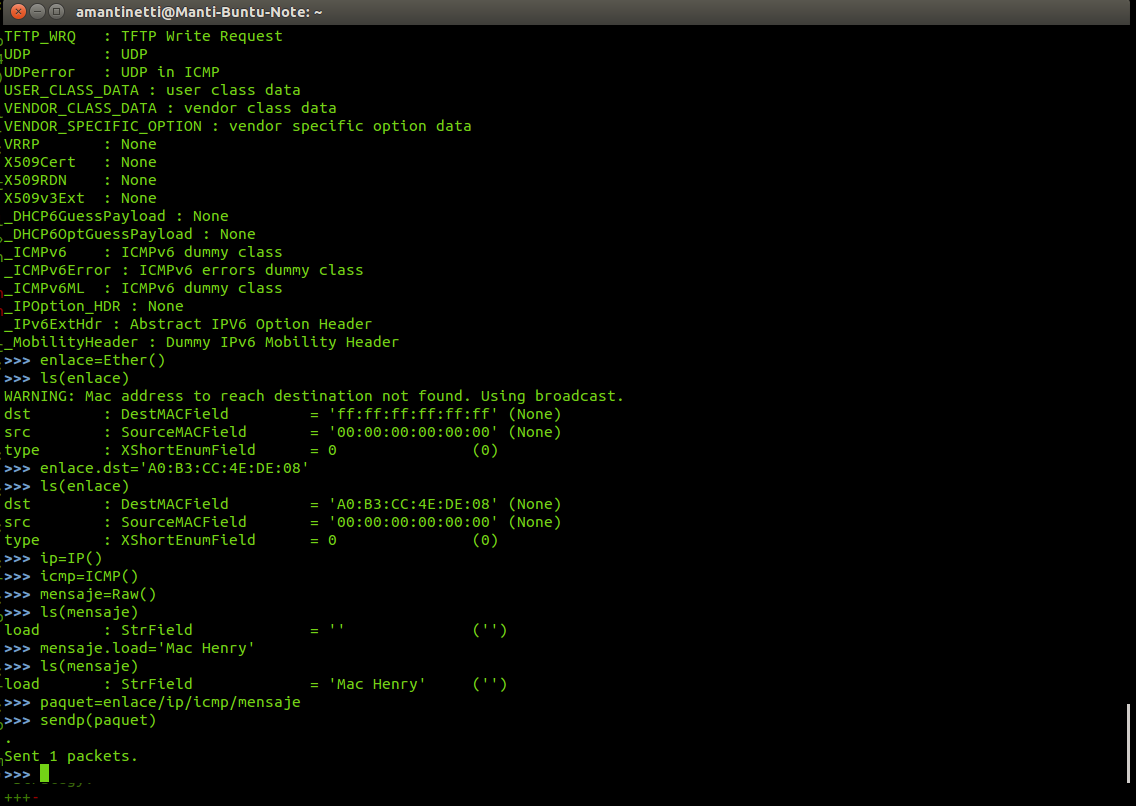
\includegraphics[scale=.27]{imagenes/Hub/sendmanti.png}
	\\
\end{center}

Luego se busca el paquete en Wireshark para ver si se envió correctamente y llegó a destino.\\

\begin{center}
	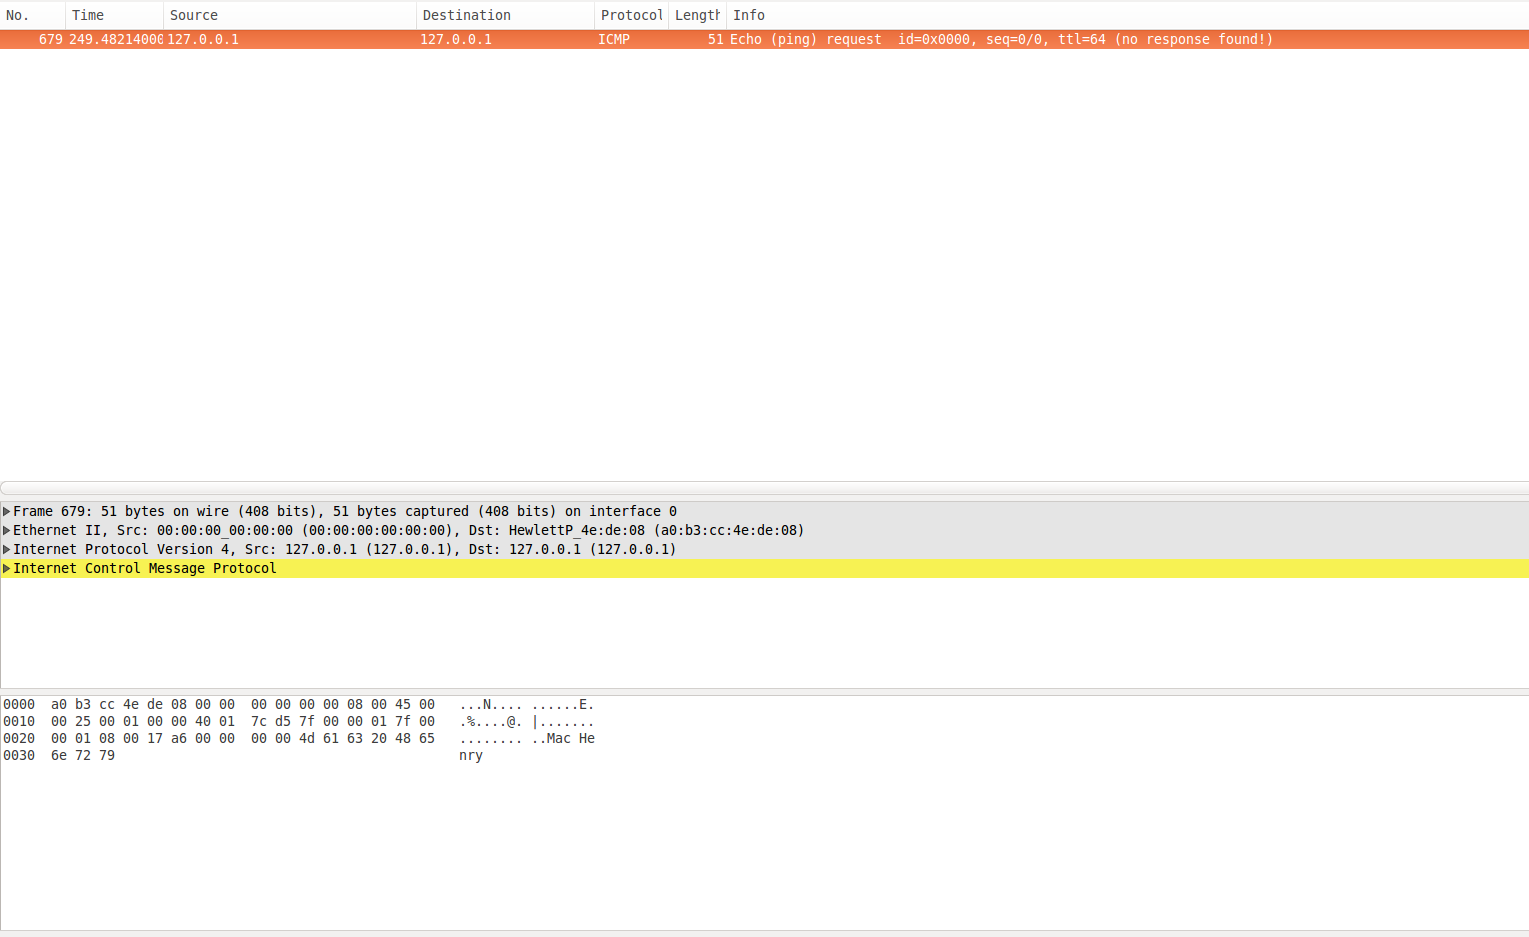
\includegraphics[scale=.27]{imagenes/Hub/ipmanti.png}
\end{center}

Confirmando que el paquete llego a destino como debería.

\pagebreak

\section{Envió de un paquete de datos con una MAC fuera de la red}

En esta ocasión se utilizo una dirección MAC de destino escrita al azar que no coincidiera con la de ninguno de los equipos pertenecientes a la red LAN. Luego se creó un paquete tras haber agregado un mensaje en la última capa, sin ningún cambio adicional el paquete fue enviado a la dirección ya mencionada.


\subsection{Switch}

La dirección MAC elegida fuera de la red para enviar el paquete fue '78:E4:00:BB:23:23'

\begin{center}
	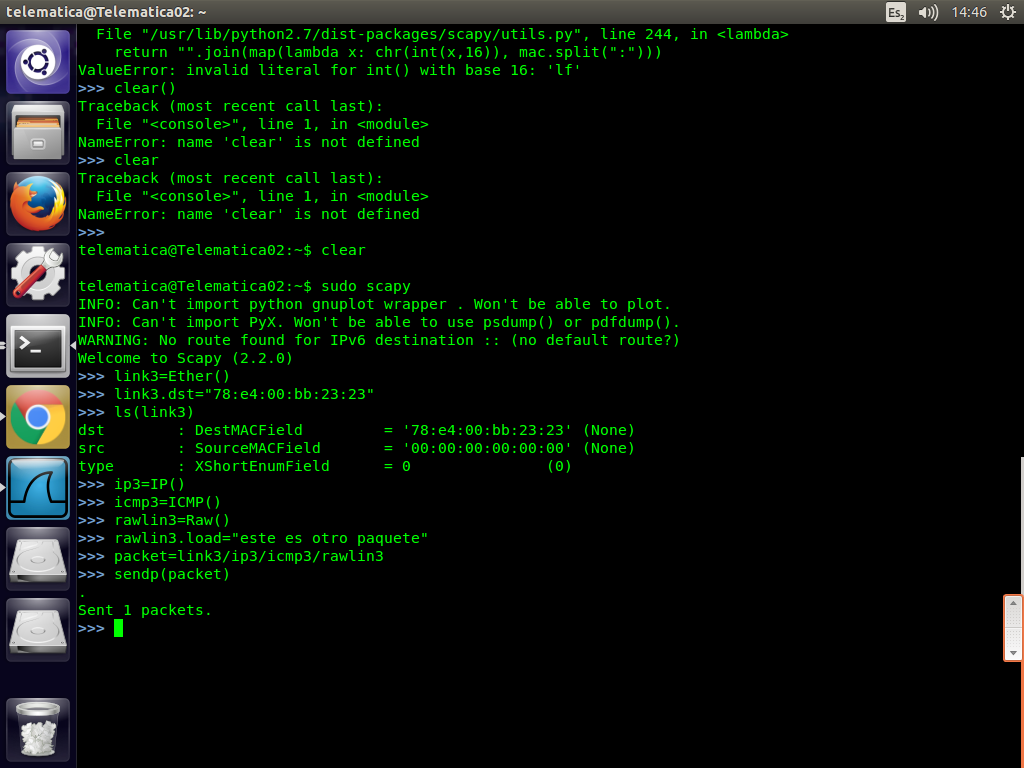
\includegraphics[scale=.37]{imagenes/Switch/Test_3.png}
\end{center}

Se descubrió que el paquete no era recibido por ninguno de los equipos.

\begin{center}
	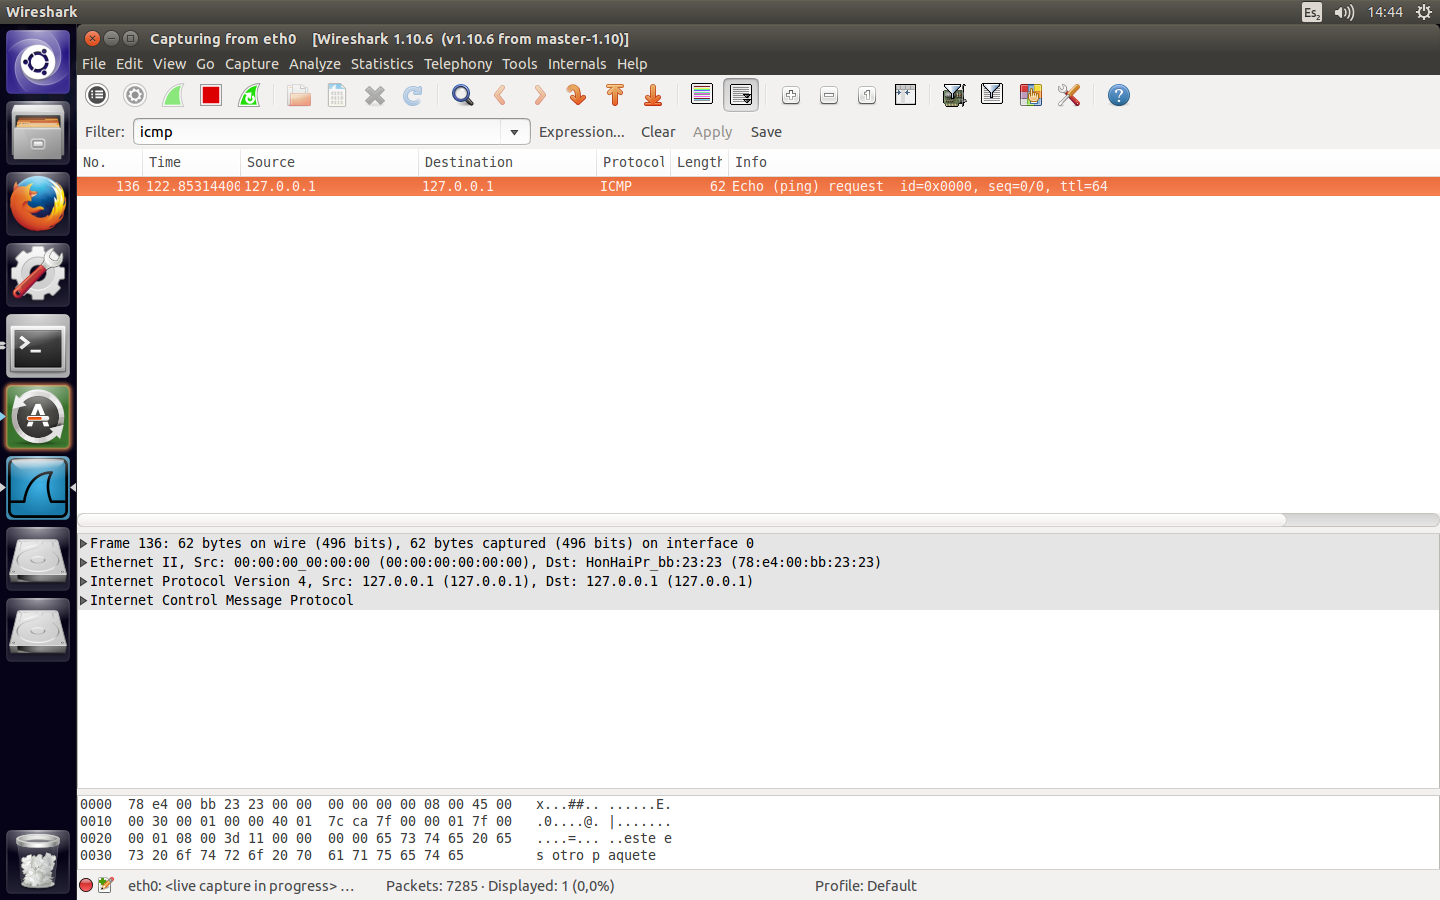
\includegraphics[scale=.27]{imagenes/Switch/Test_3_Wireshark.png}
	\\ Wireshark corriendo en modo Promiscuo para comprobar el envió del paquete
\end{center}

\newpage


\subsection{Hub}

La dirección MAC elegida fuera de la red para enviar el paquete fue 'AA:BB:CC:4E:DE:08'

\begin{center}
	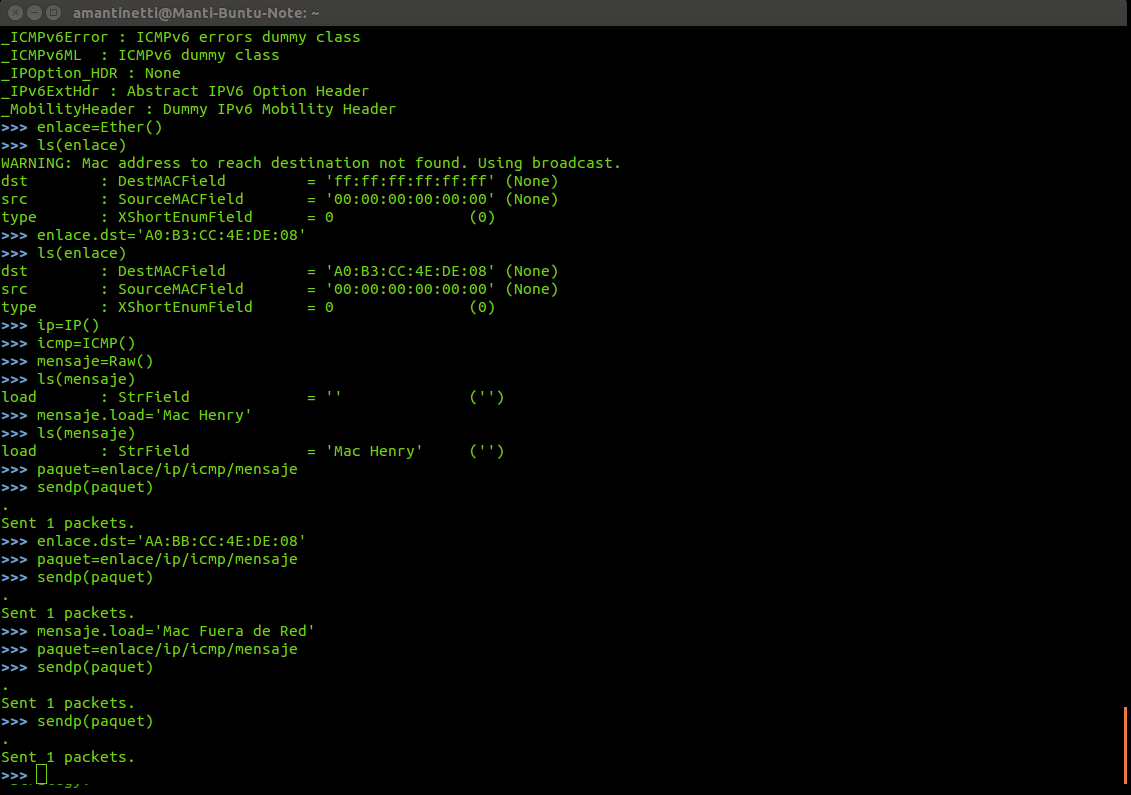
\includegraphics[scale=.27]{imagenes/Hub/consoleout.png}
\end{center}

Este paquete era recibido por todos los equipos conectados al Hub

\begin{center}
	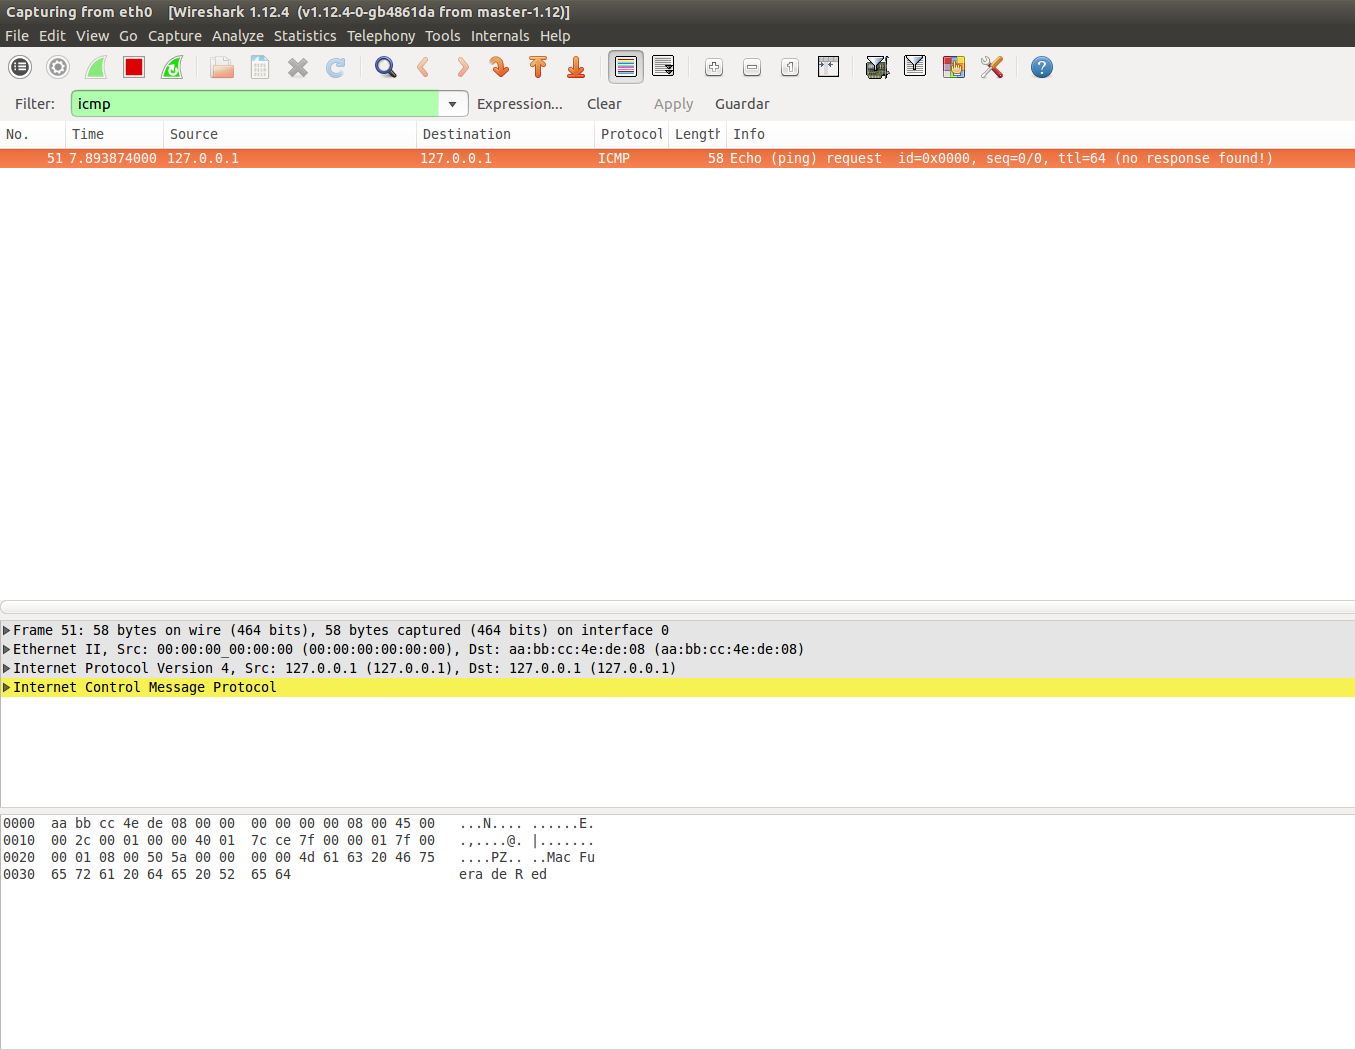
\includegraphics[scale=.27]{imagenes/Hub/wireout.png}
	\\ Wireshark corriendo normalmente 
\end{center}

\chapter{Conclusión}
Se puede observar que el hub envía todos los paquetes a todos los equipos conectados a la red, mientras que el switch los  envía según la MAC del equipo o la dirección IP. Debido a esto, se concluye que el este es más seguro que el primero a la hora de enviar paquetes por la red.
%A partir de la creación de paquetes de datos logramos comprender.....

\end{document}